\section{Montage}

Jane a réalisé le circuit électrique ci-dessous :

\begin{center}
	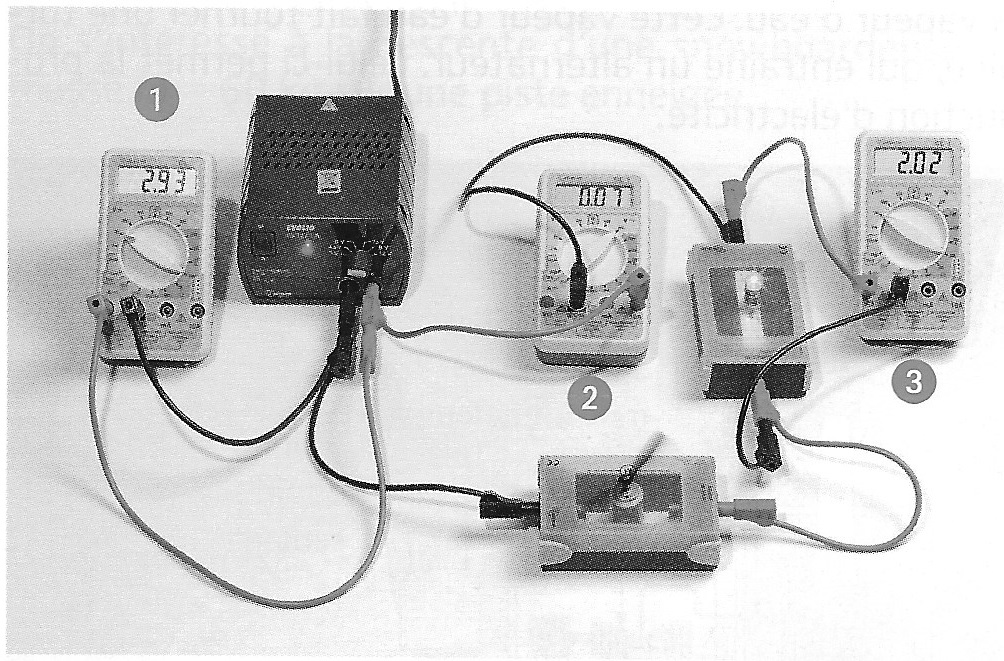
\includegraphics[scale=1.1]{img/montage_serie}
\end{center}

\begin{questions}
	
	\question 
		\begin{parts}
			\part Quels sont les appareils de mesure branchés en série ? en dérivation ?
			\fillwithdottedlines{2cm}
			\part Lesquels sont utilisés en voltmètre ? en ampèremètre ?
			\fillwithdottedlines{2cm}
		\end{parts}
	
	\question Réaliser le schéma normalisé du circuit de Jane.
	\makeemptybox{5.5cm}
	
	\question Quelles sont les tensions aux bornes :
	\begin{parts}
		\part du générateur ?
		\fillwithdottedlines{1.5cm}
		\part de la lampe ?
		\fillwithdottedlines{1.5cm}
		
		\part du moteur ?
		\fillwithdottedlines{1.5cm}
	\end{parts}

	\question Quelle est l'intensité du courant traversant :
	\begin{parts}
		\part la lampe ?
		\fillwithdottedlines{1.5cm}
		
		\part le moteur ?
		\fillwithdottedlines{1.5cm}
	\end{parts}

\end{questions}